\documentclass[a4paper]{article}
\usepackage{amsmath,amsfonts,amssymb,amsthm,mathrsfs,bm}
\usepackage{setspace}		%行间距
\usepackage{geometry}		%页边距
\geometry{left=3.18cm,right=3.18cm,top=2.54cm,bottom=2.54cm}
\usepackage{indentfirst}		%首行缩进
\usepackage[UTF8]{ctex}		%中文
\usepackage{pifont}		%带圈数字 \ding{172}
\usepackage{graphicx}		%插图 \includegraphics[width=1cm]{picture.jpg}
\usepackage{wrapfig}
\usepackage[linkcolor=black,citecolor=black]{hyperref}		%超链接
\usepackage{array}
\usepackage{float}
\usepackage{booktabs}		%\toprule \midrule \bottomrule
\usepackage{multicol}
\newcommand{\tabincell}[2]{\begin{tabular}{@{}#1@{}}#2\end{tabular}}		%表格多行显示

\usepackage{boxedminipage}
\usepackage{booktabs}
\usepackage{tabularx}

\newtheorem{thm}{\heiti 定理}
\newtheorem{prop}[thm]{\heiti 命题}
\newtheorem{defn}[thm]{\heiti 定义}
\newtheorem{exmp}[thm]{\heiti 例}
\newtheorem{lem}[thm]{\heiti 引理}
\newtheorem{cor}[thm]{\heiti 推论}
\newtheorem{rem}[thm]{\heiti 注}


\usepackage{listings}
\usepackage{fontspec}
%\newfontfamily\SF{SFMono-Regular}
\usepackage{xcolor}
\definecolor{mygreen}{rgb}{0.176,0.537,0.141}
\definecolor{myblue}{rgb}{0.031,0.016,0.933}
\definecolor{myred}{rgb}{0.698,0.153,0.125}
\definecolor{mypurple}{rgb}{0.620,0.149,0.918}
\lstset{
frame=shadowbox,
basicstyle=\footnotesize\SF,     % size of fonts used for the code
numbers=left,
numberstyle=\scriptsize\SF,
backgroundcolor=\color{white},      % choose the background color
showspaces=false,               % show spaces adding particular underscores
showstringspaces=false,         % underline spaces within strings
showtabs=false,                 % show tabs within strings adding particular underscores
tabsize=5,                      % sets default tabsize to 2 spaces
captionpos=b,                   % sets the caption-position to bottom
breaklines=true,                % sets automatic line breaking
breakatwhitespace=false,        % sets if automatic breaks should only happen at whitespace
columns=fullflexible,
escapeinside={\%*}{*)},        % if you want to add LaTeX within your code
commentstyle=\color{mygreen}\SF,  % comment style
keywordstyle=\color{myblue}\SF,     % keyword style
stringstyle=\color{mypurple}\SF,  % string literal style
rulesepcolor=\color{red!50!green!50!blue!50},
}

\begin{document}
\setlength{\parindent}{2em}
\setcounter{page}{0}
\thispagestyle{empty}
\begin{spacing}{3}
\begin{figure}[htp]
\centering

\includegraphics[width=10.6cm]{beihang2.jpg}
\end{figure}

\begin{figure}[htp]
\centering

\includegraphics[width=3.05cm]{beihang1.jpg}
\end{figure}

\bigskip

\begin{center}
{\heiti  \zihao{1} 《随机过程》大作业}

\vspace{3cm}

{\heiti  \zihao{3} 基于知乎大V的社交网络分析}
\end{center}
\end{spacing}

\vspace{2cm}

\begin{spacing}{2.25}
\begin{center}

{\heiti \zihao{4} 院系名称:}\underline{\makebox[8cm]{\fangsong\zihao{-4} 数学与系统科学学院}}

{\heiti \zihao{4} 小组成员:}\underline{\makebox[8cm]{\fangsong\zihao{-4} 15091060\quad 张{\color{white}一}晋\qquad 15091056\quad 王兴坤}}

{\heiti \zihao{4} {\color{white} 小组成员:}}\underline{\makebox[8cm]{\fangsong\zihao{-4} 15091034\quad 廖星晔\qquad 15091045\quad 宋萌萌}}

{\heiti \zihao{4} {\color{white} 小组成员:}}\underline{\makebox[8cm]{\fangsong\zihao{-4} 15091052\quad 涂宇彬\qquad 15091017\quad 刘勇晟}}




\vspace{2.5cm}

{\heiti  \zihao{4} 2018年6月}
\end{center}
\end{spacing}



\newpage
\begin{spacing}{1.5}
\thispagestyle{empty}
\tableofcontents
\setcounter{page}{1}
\thispagestyle{empty}


\newpage
\setcounter{page}{1}
\begin{spacing}{2.25}
\begin{center}
{\heiti  \zihao{3} 序言}
\end{center}
\end{spacing}
本文分8节。第~\ref{sec1}~节是问题背景,介绍了知乎并说明我们的目的;
第~\ref{sec2}~节说明我们是如何获取知乎大V社交网络数据并将其可视化的;
然后在第~\ref{sec3}~节中,我们从网络的规模、密度、连通性、度分布等角度对这个社交网络的结构进行了详细地分析,说明了这个网络具有高聚类性和短路径性等小世界特性,而且这个网络用
户之间联系非常紧密;
在第~\ref{sec4}~节中,我们通过不同的中心性指标来从三个角度衡量用户对网络的重要程度,最终找出了这个网络的核心人物——黄继新;
在第~\ref{sec5}~节中,我们介绍了 PageRank 算法,使用该算法通过邻接矩阵对知乎用户进行排序,最后排名第一的大V还是黄继新;
在第~\ref{sec6}~节中,我们对PageRank 算法与另外三种中心度指标进行比较,发现总体上成正相关,说明PageRank值可以作为节点中心度指标的一种综合衡量。
最后在第~\ref{sec7}~节中,我们通过用户信息来分析 PR 值较高的用户有哪些特征,发现知乎大V们从事比例最高的行业为互联网,并且都在自己的专业领域里有着扎实的基础,能将复杂的专业知识用生动的语言普及给大众。
\section{问题背景}\label{sec1}
作为国内最大的在线问答社区——知乎,相信大家并不陌生,
它与百度知道等其他问答网站最大的不同是,知乎更强调社交性,用户通过提出和回答问题、关注、赞同等方式构建社区人际关系。相比于“有社交属性的问答网站”,知乎倒更像一个“以问答为主的社交网站”。因此其浓厚的社交属性非常适合用于社交网络分析。

而知乎社区的运行机制中的投票机制和关注机制又必然导致意见领袖的产生,也是我们俗称的大V。我们想知道在这些大V组成的圈子中,哪些人起着举足轻重的作用,也就是说,我们想找出谁才是大V中的大V。

\section{社交网络数据的获取及可视化}\label{sec2}
\subsection{爬取数据}
我们通过Python程序爬取了知乎被关注数最高的200个大V的信息(见图~\ref{info1},具体数据见Excel文件 \verb"Info_2018_5_26.xlsx"),并根据\textbf{他们之间相互关注的
关系}构成了一个有向的社交网络。

由于知乎没有官方的API,所以如果要获得精确的前200个被关注数最高用户就必须爬取绝大部分知乎用户,由于编程能力和时间限制,我们只能以知乎用户\href{https://www.zhihu.com/people/sgai/activities}{路人甲}在2016年12月爬取的数据为基础,根据用户昵称重新搜索数据,并根据被关注数重新排序确定最终结果。由于可能有大V在这期间改名,或者有新的大V强势崛起,所以可能结果并不是精确信息,但对社交网络分析没有太大影响。


\subsection{具体过程}
首先将已有用户名存到文件 \verb"User_name.txt" 中,
  然后运行程序  \verb"Token_url_search.py" 对该文件中的用户名进行搜索,在同名用户中找到被关注数最多的那个用户,记录其用户名、token\_url(每个用户可能有相同的用户名,但只有唯一一个token\_url)和被关注数。

  然后选出被关注数排名前200的用户,将其姓名重新覆盖存到 \verb"User_name.txt" 中,将其token\_url存到 \verb"User_id.txt" 中。

  通过程序 \verb"Info_search.py" 搜集这些用户的具体信息,存到文件 \verb"Info_2018_5_26.xlsx" 中。

  通过程序 \verb"Link_search.py" 搜速这些用户间的互相关注信息,并构建关系矩阵储存到 \verb"Link_mat.xlsx" (含用户名,以便查看)和 \verb"link.csv" (不含用户名,纯矩阵,方便程序调用)。
\begin{figure}[H]
  \centering
  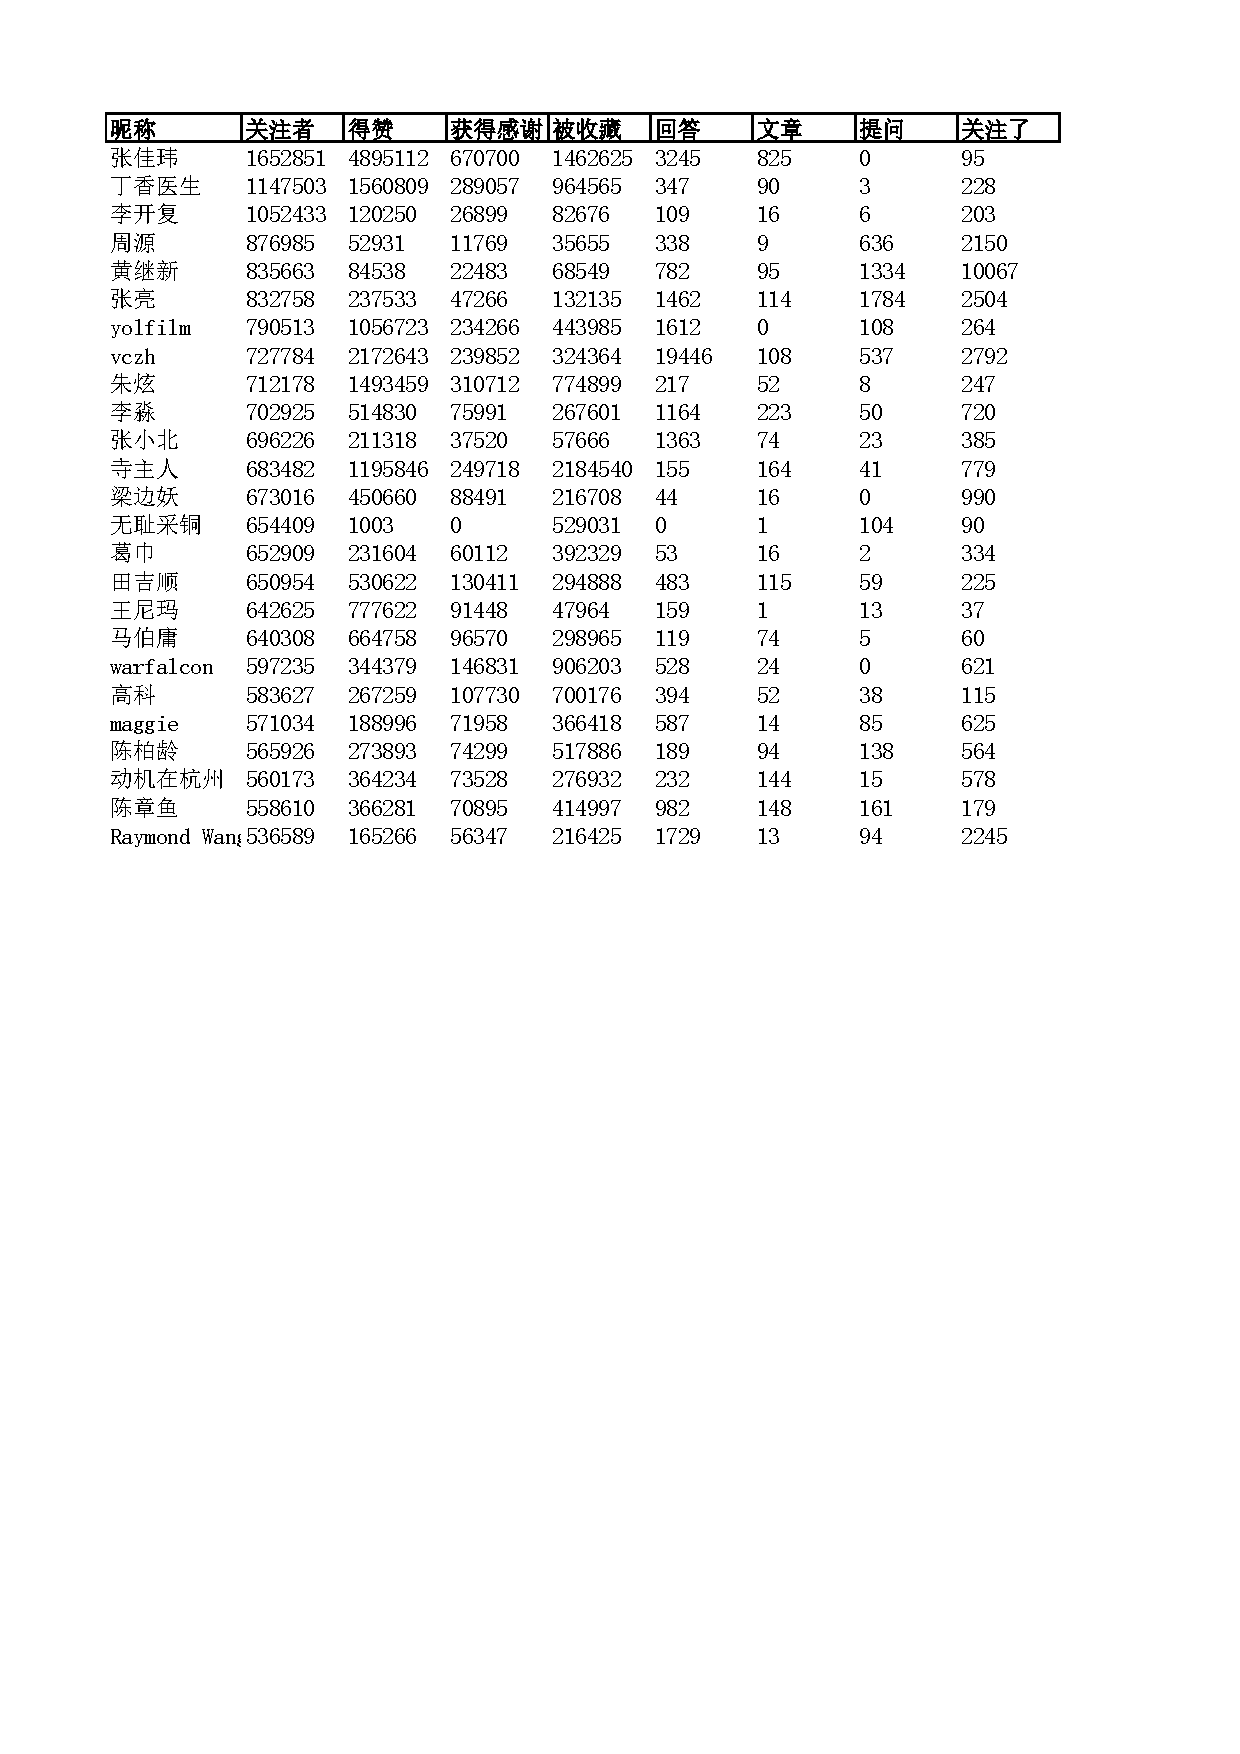
\includegraphics[width=14cm]{fig/info_1.pdf}
  \caption{部分大V信息}\label{info1}
\end{figure}
\subsection{社交网络可视化}
\subsubsection{通过NetDraw可视化社交网络}
我们将邻接矩阵\verb"Link_mat.xlsx"输入到UCINET6中,获得了Ucinet databset network文件\verb"Link_mat.##h",然后导入到NetDraw2.161绘制这200个大V构成的社交网络图,见图~\ref{netjpg}。
\begin{figure}[H]
  \centering
  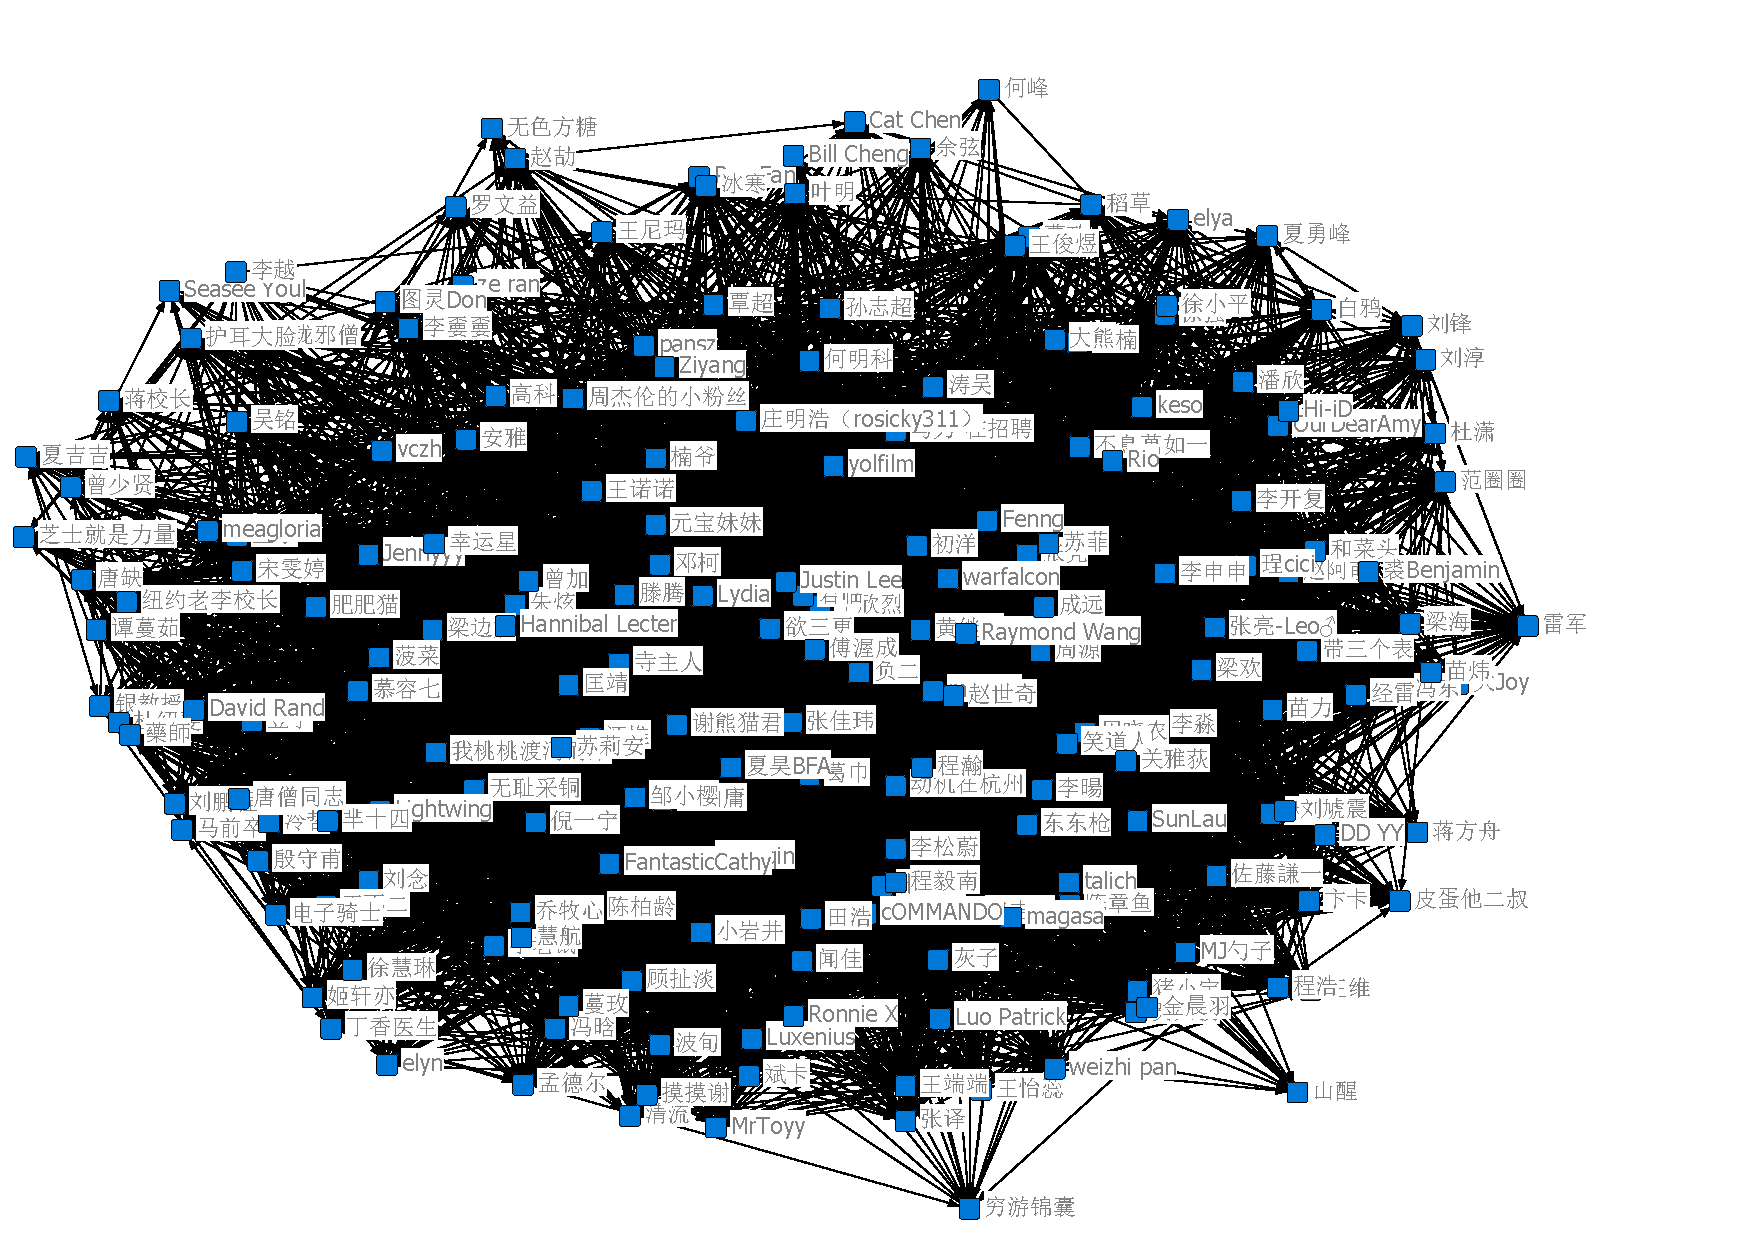
\includegraphics[width=12cm]{fig/net200.pdf}
  \caption{知乎大V社交网络图}\label{netjpg}
\end{figure}

为了使图像看起来更清晰,我们又选取前50个大V的关系图进行绘制(见图~\ref{net50jpg})。
\begin{figure}[H]
  \centering
  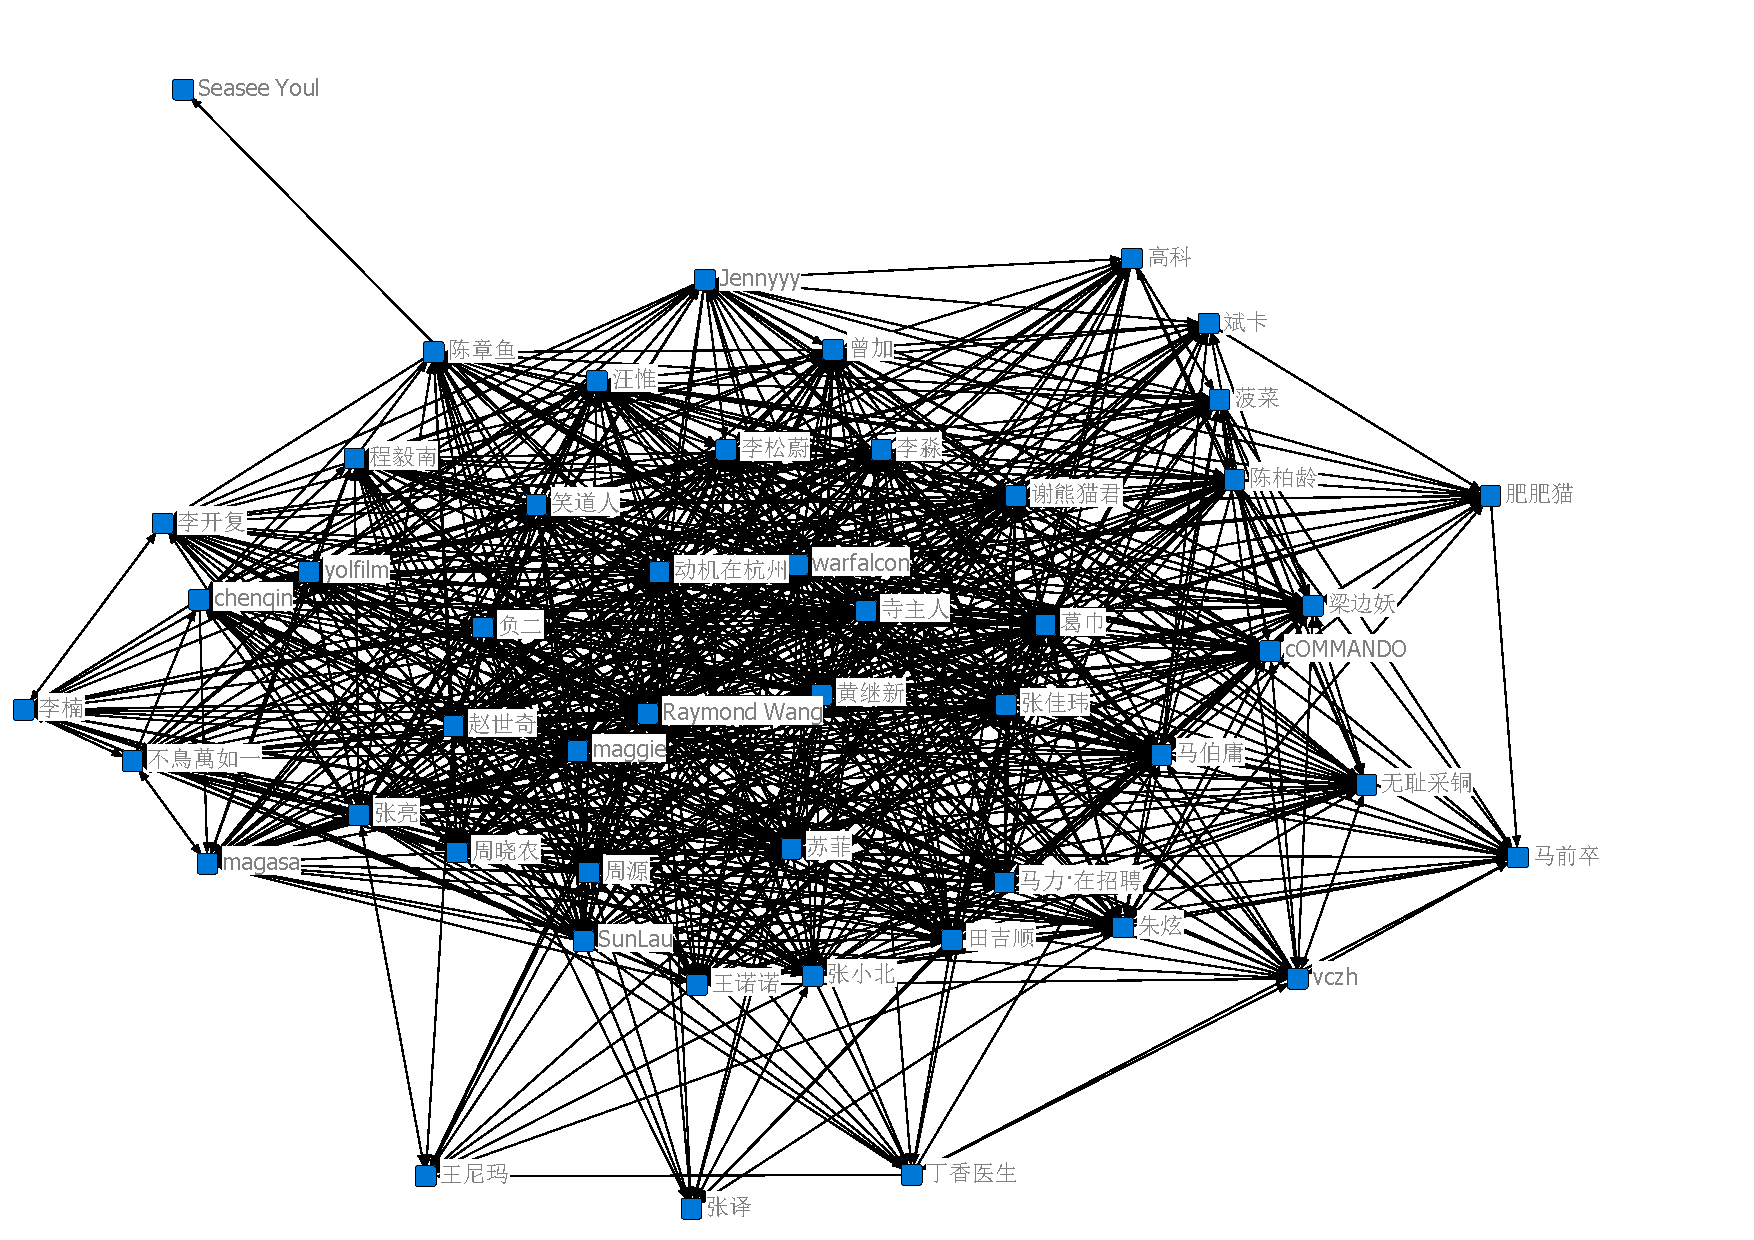
\includegraphics[width=14cm]{fig/net50.pdf}
  \caption{前50大V社交网络图}\label{net50jpg}
\end{figure}

\subsubsection{通过D3可视化社交网络}
D3.js(Data-Driven Documents)是一个JavaScript库,用于在Web浏览器中生成动态的交互式数据可视化。

我们在\url{https://github.com/d3/d3/wiki/gallery}上找了一个捆图(Hierarchical Edge Bundling)的脚本模板,用程序\verb"json_generator.py"根据用户关系产生相应的json文件,然后载入到网页中即可,具体效果见图~\ref{100}。

我们将网页上传到了GitHub上,预览链接如下:
\url{http://htmlpreview.github.io/?https://github.com/Theigrams/seezhihu/blob/master/bundle1.html}

因为关系太紧密,所以可能有有所卡顿,我们又选取了前50个大V来观察,链接如下:\url{http://htmlpreview.github.io/?https://github.com/Theigrams/seezhihu/blob/master/bundle2.html}

将鼠标移到用户的名字上时,就会显示出他关注和被关注的人。红线表示关注他的人,绿线表示他关注的人,如果是互相关注了的话还是用红线表示。

tension表示使线条弯曲的拉力,越靠左线条越直,弯曲程度越弱。

\begin{figure}[htp]
  \centering
  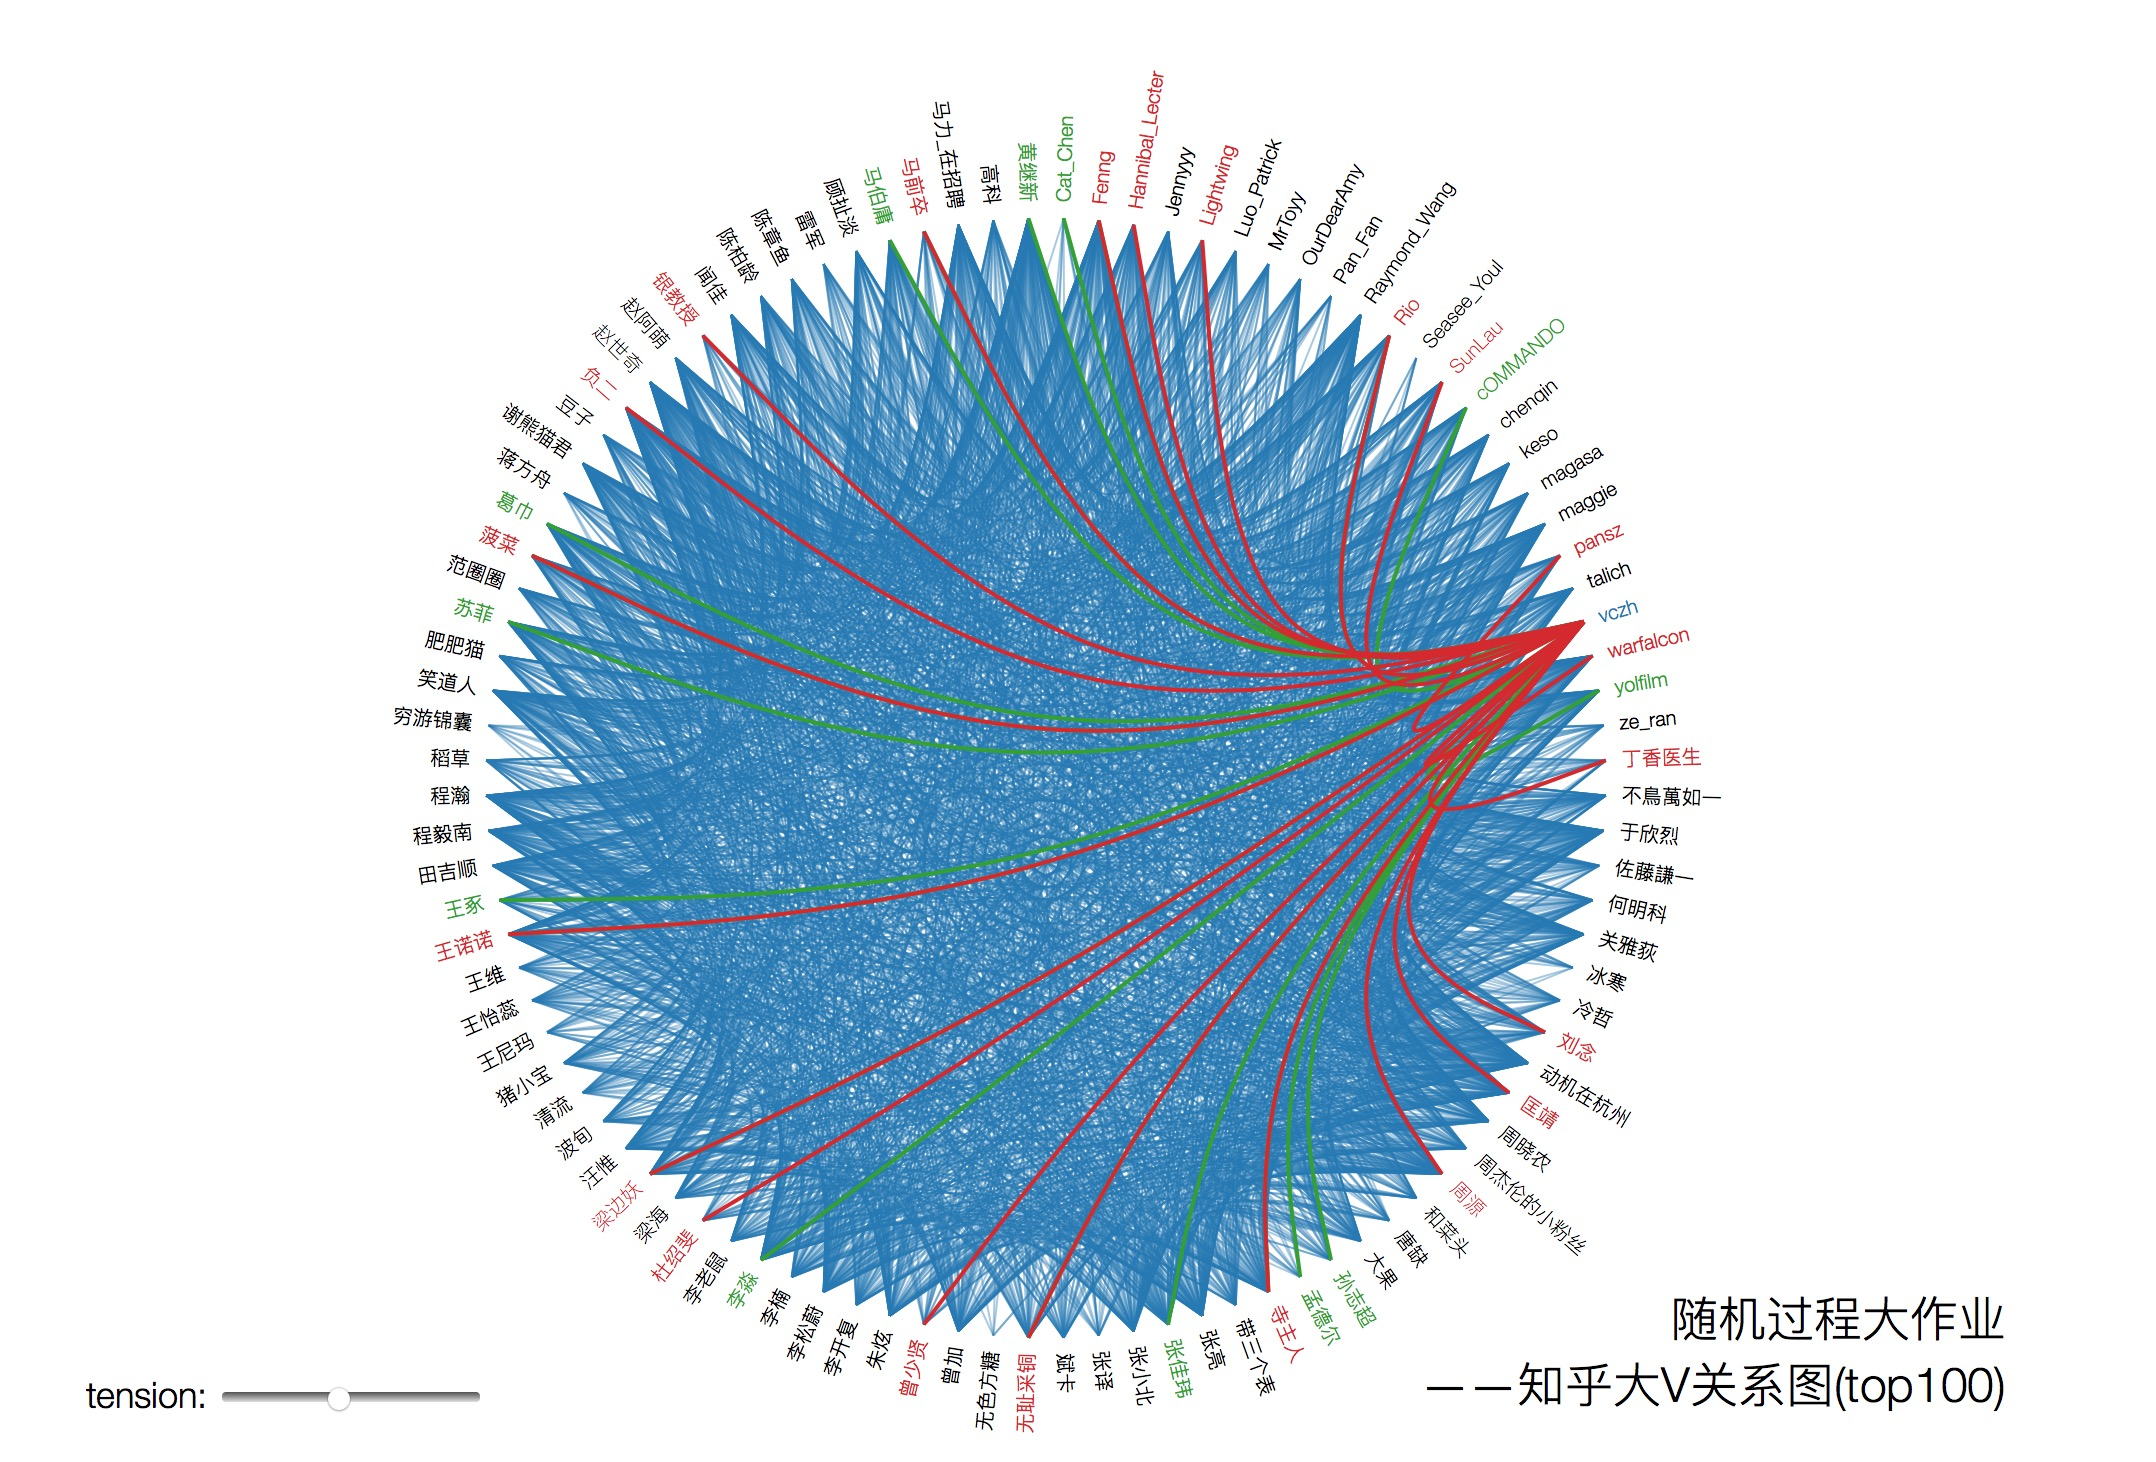
\includegraphics[width=16cm]{fig/D2.jpg}
  \caption{Top100大V关系图}\label{100}
\end{figure}


\newpage
\section{网络结构分析}\label{sec3}
\subsection{网络规模}
经统计,该社交网络中的节点数为200,连接数为10275。
\subsection{网络密度}
有向整体网的密度计算公式:
\[\text{Density}=\dfrac{m}{n(n-1)}\]
其中$m$为连接数,$n$为节点数,$n(n-1)$为理论最大连接数。

经计算得该网络的密度为0.2582,网络连接的标准差为0.438。整体密度较高,说明用户之间联系非常紧密。

\subsection{网络平均度}
所有节点的度的平均值称为网络的平均度(Average Degree),当给定网络的邻接矩阵$\mathbf{A}$时,其计算公式如下:
\[\langle k\rangle=\dfrac{1}{N}\sum_{i,j=1}^{N}a_{ij}\]

经计算得,该网络的平均度为51.375。

\subsection{平均路径长度}
网络的平均路径长度$L$定义为任意两个节点之间的距离的平均值,即
\[L=\dfrac{2}{n(n-1)}\sum_{i\geq j}d_{ij}\]

经计算得:平均距离= 1.767,基于距离的凝聚力(“紧密度”)= 0.619(范围从0到1,较大的值表示较大的凝聚力)

\begin{table}[H]
\centering
\caption{路径频率}
\label{path}
\begin{tabular}{cc}
  \toprule
  \qquad 路径长度\qquad  & \qquad 频率 ~~~~\qquad  \\
  \midrule
  \qquad 1 & \qquad 0.261  ~~~~\qquad \\
  \qquad  2 & \qquad 0.711  ~~~~\qquad \\
  \qquad  3 & \qquad 0.028  ~~~~\qquad \\
  \bottomrule
\end{tabular}
\end{table}

由表\ref{path}可知,在这个社交网络中99.7\%的用户只需通过中间两个人就能建立起联系。


\newpage
\subsection{连通性分析}
对于这个巨大的社交网络,我们希望知道它的连通性情况。

我们现在拥有这个社交网络的邻接矩阵,$a_{ij}=1$表示走一步可以从节点$i$到达节点$j$,那么$\sum_{k=1}^{N}a_{ik}a_{kj}$表示走两步能从节点$i$到达节点$j$的路径数,那么如果走了$n$步后从节点$i$到达节点$j$的路径数就是$(A^n)_{ij}$,那么无论走多少步都无法从节点$i$到达节点$j$体现为$\hat{A}_{ij}=0$,其中
\[\hat{A}={A + {A^2} +  \cdots  + {A^n} +  \cdots=(I - A)^{ - 1}} - I\]

为了防止矩阵相乘导致精度溢出,我们先将邻接矩阵进行预处理,将每一行归一化,然后进行计算。

最终这样我们通过观察数据,除了\verb"无色方糖"与\verb"芝士就是力量"这两人不能到达别的节点,其余节点都是强连通,且都可以到达这两点,也就是两点以外属于强连通核,该两人属于网络的出部。

\subsection{网络的度分布}
我们可以把网络中节点的度按从小到大排序,从而统计得到度为$k$的节点占整个网络节点数的比例$p_k$。从概率统计的角度来看,$p_k$也可以视为网络中一个随机选择的节点的度为$k$的概率,这就是\textbf{度分布}(Degree distribution)的概念。

%对于无向网络,其度分布$P(k)$定义为网络中一个随机选择的节点的度为$k$的概率。对于有向网络,则分为出度分布与入度分布。出度分布$P(k^{out})$定义为网络中随机选取的一个节点的出度为$k^{out}$的概率,入度分布的定义类似。

\subsubsection{两种分布曲线}

网络度分布可能呈现两种曲线形状不同的分布——正态分布与长尾分布。
\begin{figure}[htp]
  \centering
  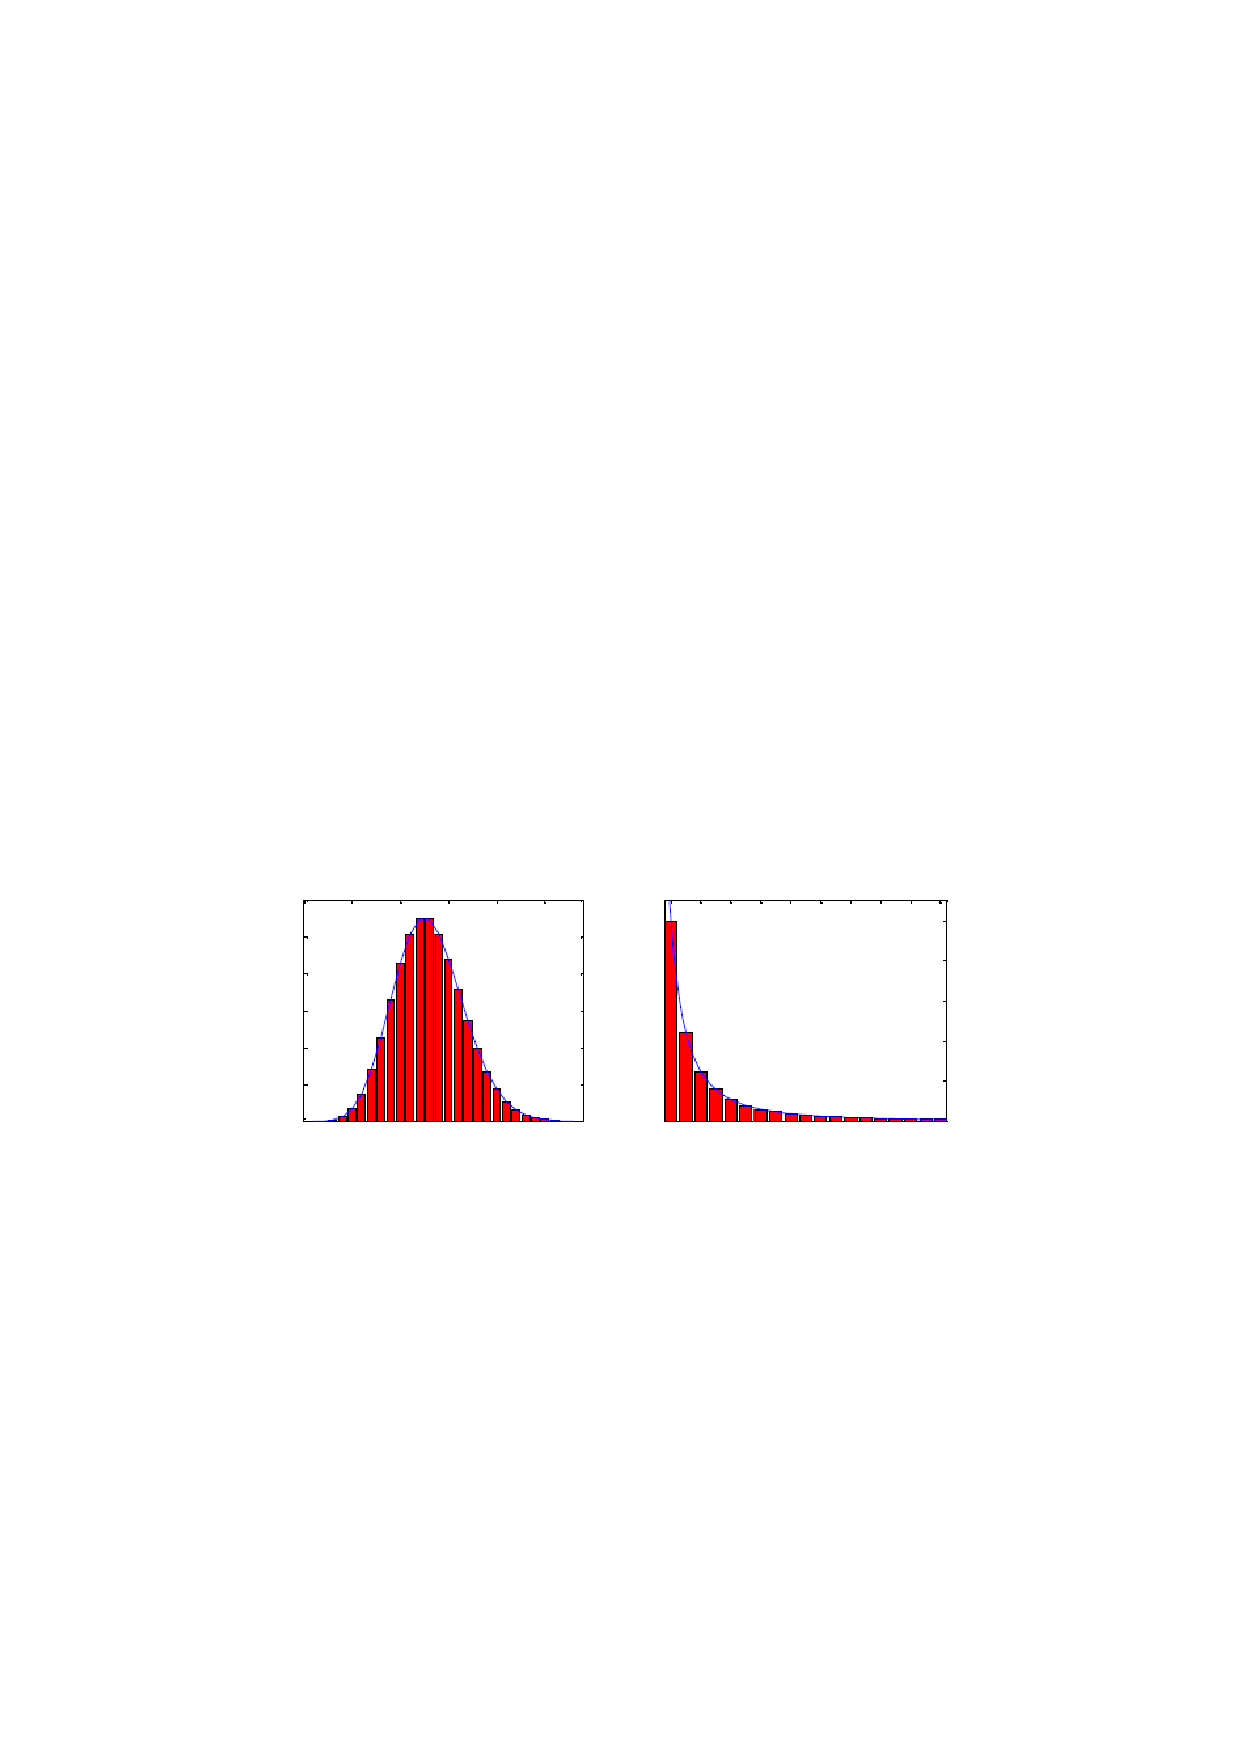
\includegraphics[width=8cm]{fig/f5.pdf}
  \caption{正态分布(左)与长尾分布(右)}\label{fb}
\end{figure}

%正态分布是最常见、最重要的概率分布,常记为$\xi \sim N(\mu , \sigma ^2)$。正态分布曲线是钟形对称曲线正态分布:均值$\mu$决定了分布的中心,标准差$\sigma ^2$决定了分布的形状。正态分布的均匀性体现在绝大部分的数据都落在均值附近。
%
%正态分布是针对连续型随机变量而言的,而网络中随机选取的一个节点的度值则是一个离散型随机变量,取值范围为非负整数。其实,常见的离散型概率分布比如超几何分布、二项分布与泊松分布等,它们在一定条件下都可以近似看作是正态分布的离散化形式,并且概率分布图都近似具有钟形形状。

服从钟形分布的随机变量具有一个明显的特征标度——钟形曲线的峰值(即随机变量的均值)。所谓特征标度是指\emph{大部分取值应该落在以特征标度为中心的一个相对比较小的区间内}。

%
%在引入长尾分布的定义之前,先介绍一个例子:考虑全球个人财富分布,容易知道这是极端不均匀的,少数人掌握着这个世界上多数的财富。联合国下属的世界发展经济学研究院2006年发布报告称,$2 \%$最富有的成年人拥有全球$50 \%$的财富,而$50 \%$最贫穷的人口仅拥有全球$1 \%$的财富。因此全球个人财富分布图呈现出与钟形曲线完全不同的形态,它会具有一个长长的尾巴,将这种分布称

长尾分布大部分个体取值较小,但是会有少数个体的取值非常大。与钟形分布存在一个明显的特征标度不同,长尾分布往往不存在单一的特征标度,因此也称为\textbf{无标度分布}。

下面回到网络度分布上,我们可以看到,如果一个实际网络的度分布曲线近似具有钟形形状,其形状在远离峰值$\langle k \rangle$处呈指数下降。这意味着我们几乎可以肯定地认为网络中所有节点的度都与网络的平均度$\langle k \rangle$相差不大。因此,这类网络也被称为均匀网络或匀质网络。然而,大量实证研究表明,许多实际网络的度分布曲线都具有长尾的性形状。

%下面我们将介绍一种具有长尾的形状的分布函数——幂律分布。幂律分布一般具有如下形式:
%\[
%P(k) \sim k^{-\gamma}
%\]
%其中$\gamma >0$为幂指数,通常取值在2与3之间。而在一定的数学意义下,幂律分布是唯一一种具有无标度特性的长尾分布。

%\subsection{幂律分布的判别方法}
%
%这里我们介绍一种判别幂律分布的判别法——双对数坐标系直线法。
%
%我们要验证是否存在比例常数$C$和幂指数$\gamma$,使得近似有
%
%\[
%P(k)=Ck^{-\gamma}
%\]
%
%可以对上式两边取对数,从而有
%
%\[
%\ln P(k) = \ln C - \gamma \ln k
%\]
%
%这说明$\ln P(k)$是$\ln k$的线性函数,也就是说,如果以$\ln k$为横轴、$\ln P(k)$为纵轴,我们应该会看到一条斜率为$-\gamma$的直线,$\ln C$为纵轴的截距。因此,直观上,若根据给定的数据,在双对数坐标系中看到近似有一条直线,那么就可以推断所处理的数据近似符合幂律,并且可以从该直线的斜率得到对应的幂指数。

\subsubsection{该社交网络的度分布}

下面我们来分析前文中构建的网络的度分布。我们首先绘制出每个用户的度从大到小排序的柱状图(见图~\ref{zzt}),可以看到,用户度之间的差异并不大,变化也很平缓。
\begin{figure}[H]
  \centering
  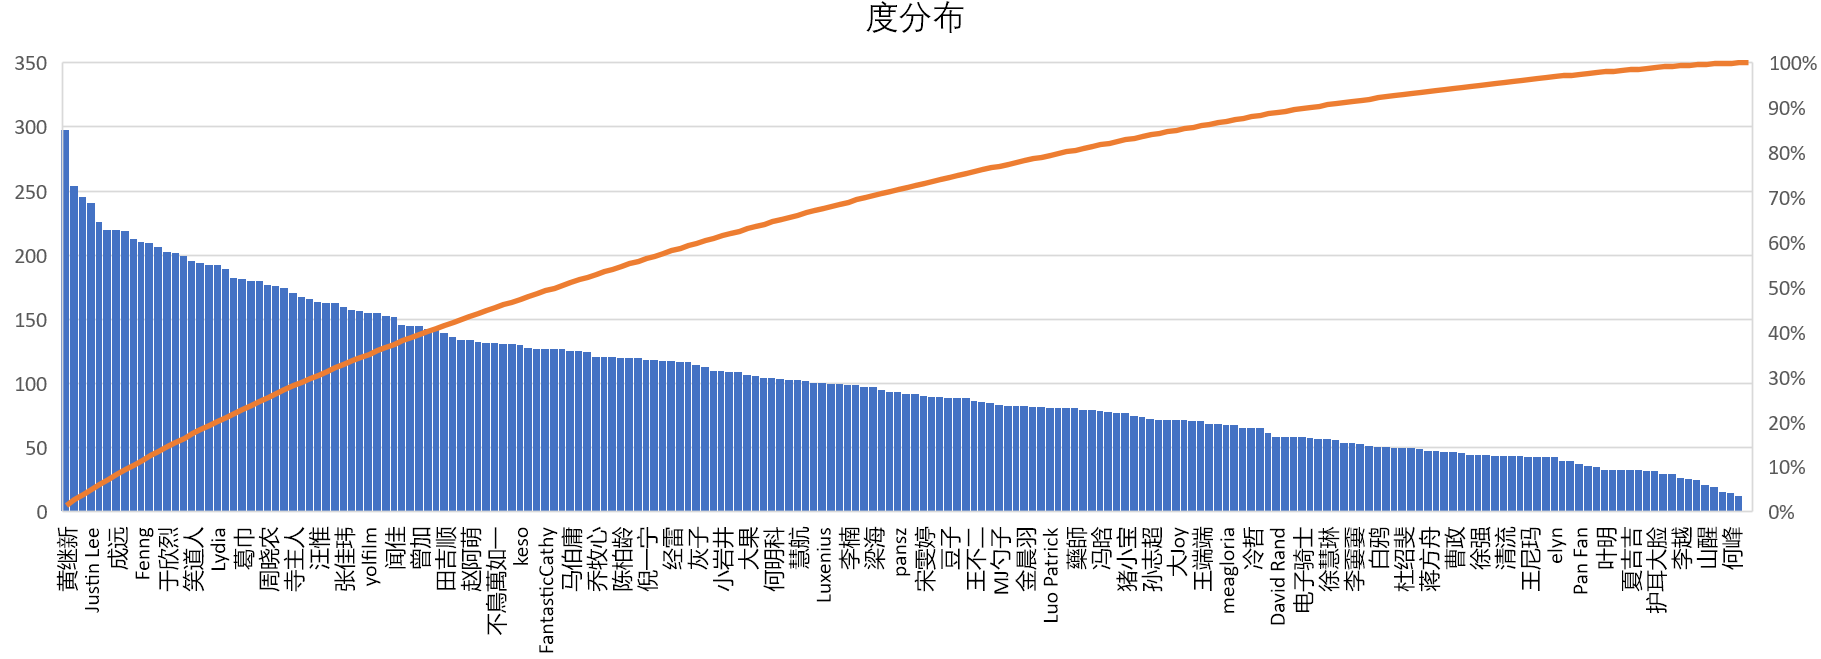
\includegraphics[width=15cm]{fig/f8.png}
  \caption{柱状图}\label{zzt}
\end{figure}
我们的网络中,节点数目较小,共200个。按照正常的操作方式得到的概率分布图像性质并不明显,因此我们想到将横轴改为间距,绘制直方图,以体现图像性质。最终我们得到图像~\ref{zft}如下:

\begin{figure}[H]
  \centering
  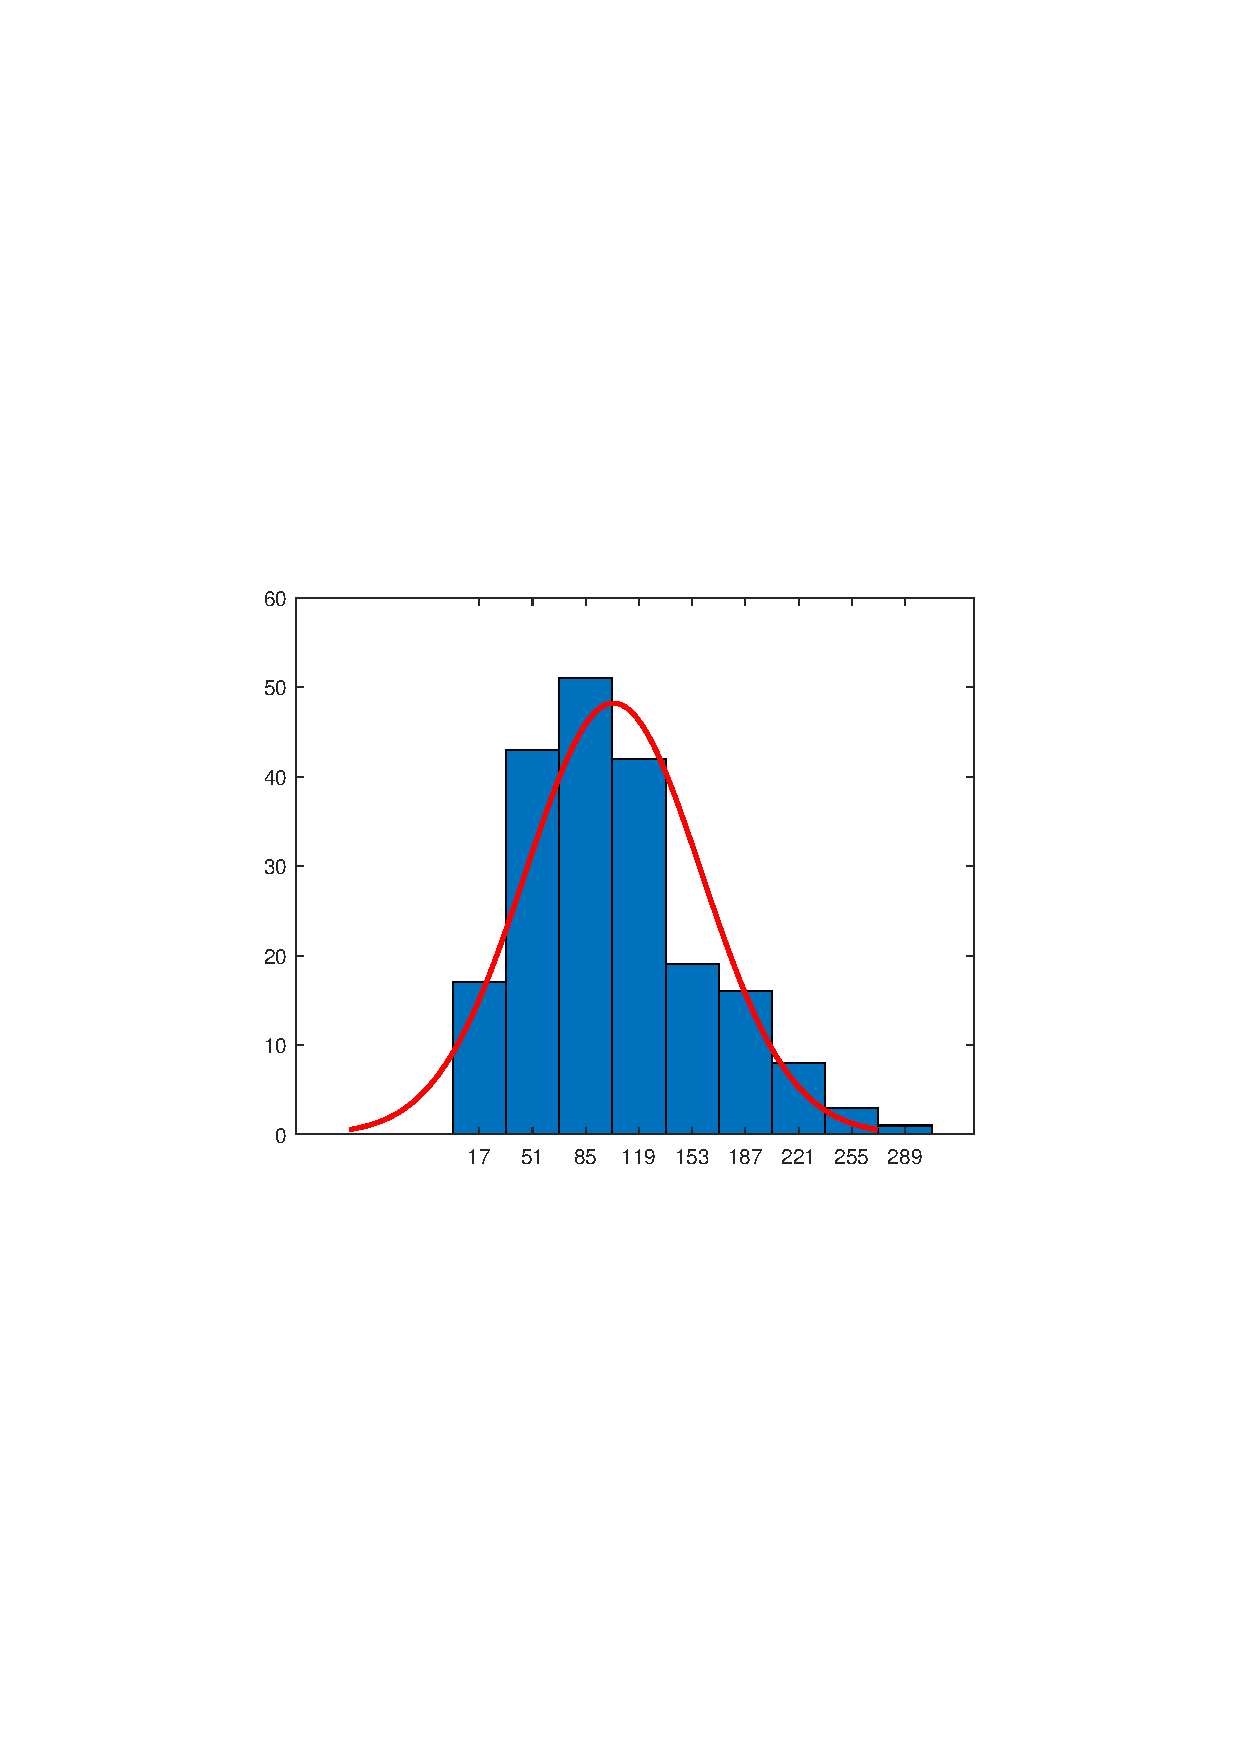
\includegraphics[width=10cm]{fig/f7.pdf}
  \caption{度分布直方图}\label{zft}
\end{figure}

可以看到,大致上是符合正态分布的,与ER随机网络的长尾分布不同,说明大V社交圈中,人与人之间不是随机去关注别人的。


\subsection{小世界特性分析}
\subsubsection{小世界含义}
完全规则网络虽然有较高的聚类特性,但不具有那么短的平均距离,而完全随机的ER随机网络虽然具有小的平均路径长度,但却没有高聚类的特性。因此完全规则网络和完全随机网络都不能再现许多实际网络——同时具有高聚类性和短平均距离。(高聚类系数在生活中的体就是“朋友圈重合”——朋友的朋友大部分还是我的朋友,短平均距离在生活中的体就是“六度分隔”——任意两个人之间只需要经过极少个人就能建立起联系)
\begin{figure}[H]
  \centering
  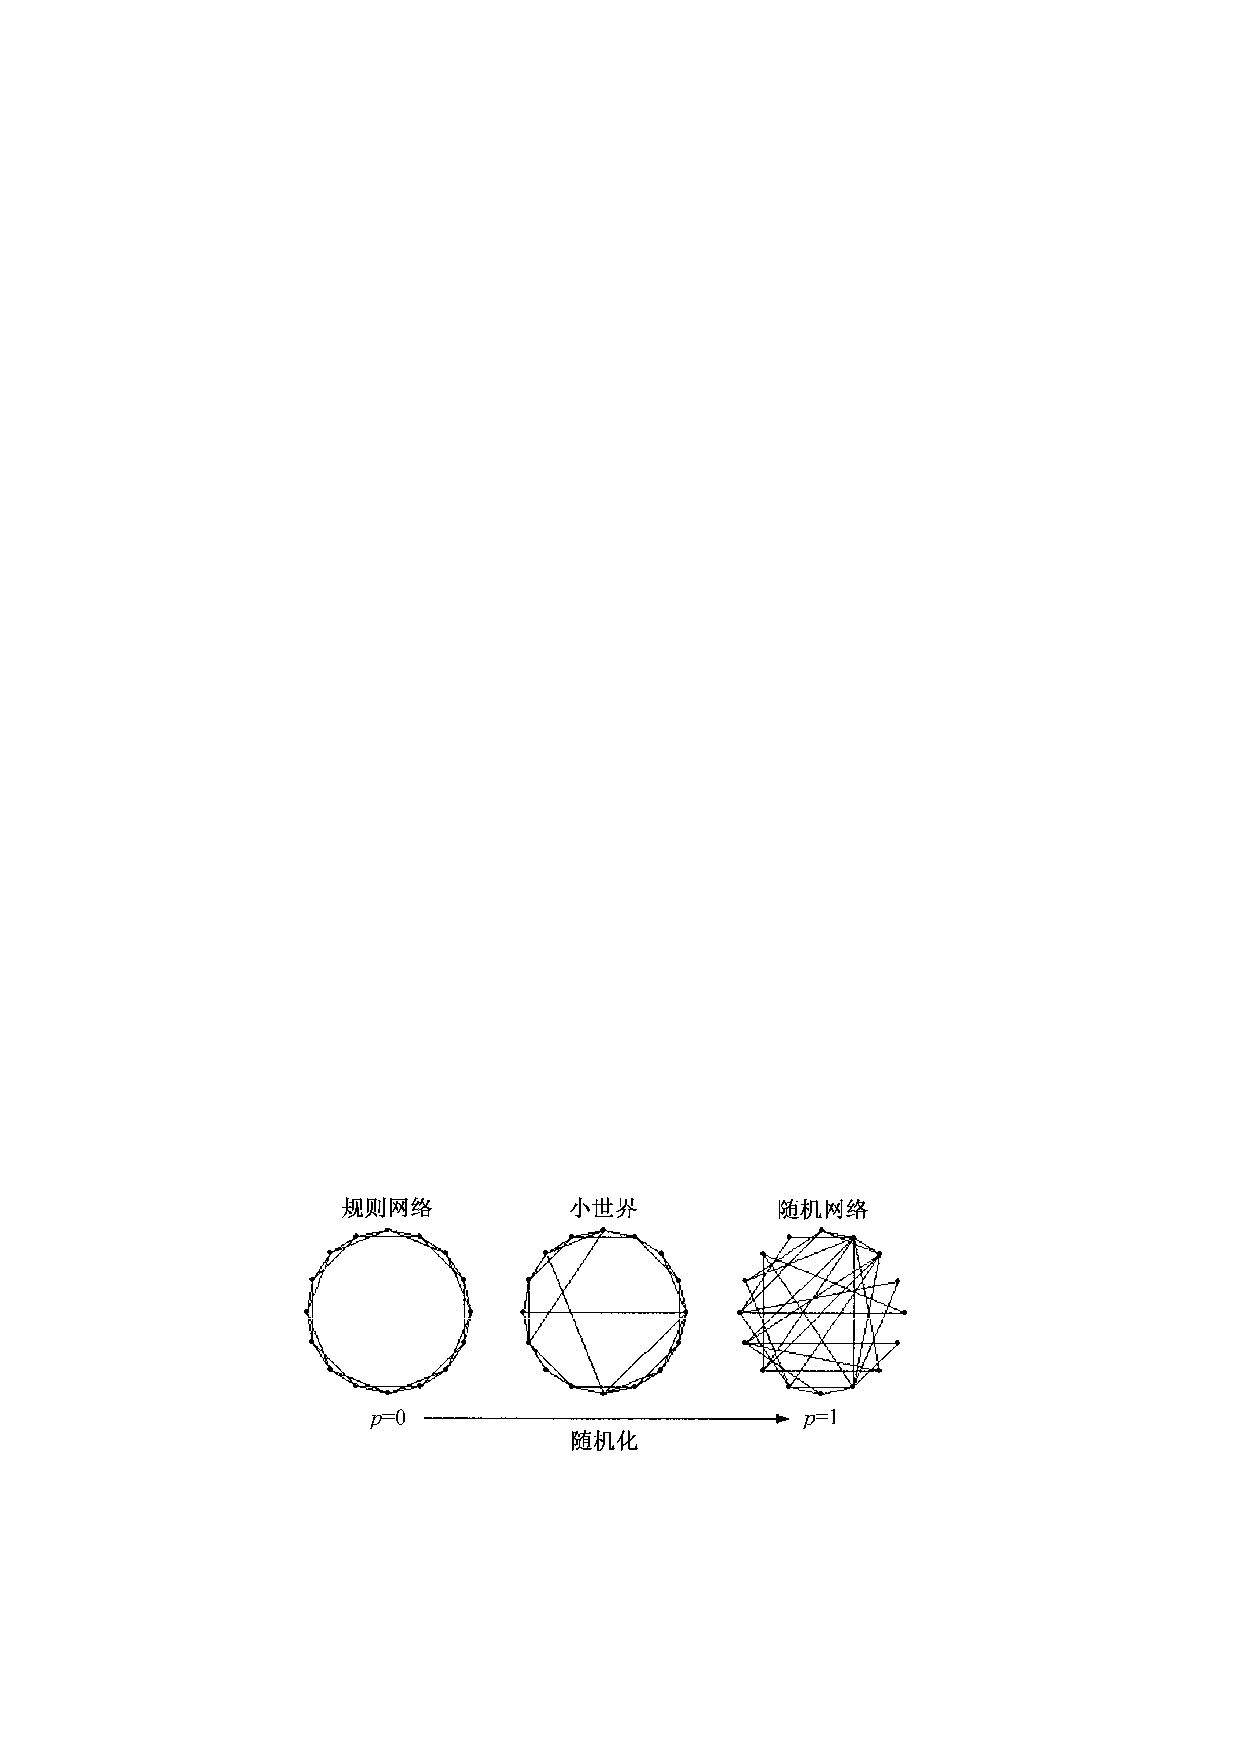
\includegraphics[width=8cm]{fig/f6.pdf}
  \caption{随机化程度介于规则网络(左)和随机网络(右)之间的WS小世界网络}\label{ws}
\end{figure}

而作为从完全规则网络向完全随机网络的过渡——小世界网络同时兼备这两种特性。在此我们不做展开,仅验证我们的社交网络是否符合小世界特性
\subsubsection{小世界性质}
我们可以利用如下两个统计量来刻画它的性质,并且以之来判断一个特定网络是否为小世界网络。
\begin{enumerate}
\item
聚类系数$C$ (Cluster Coefficient):定义为网络中所有节点的聚类系数的平均值。

\item
平均最短路径长度$L$ (Average Shortest Path):连接任何两个点之间最短途径的平均长度。
\end{enumerate}
\subsubsection{特性分析}
由于只能计算无向图的聚类系数,实验我们先将有向知乎社交网络转化为无向网络,然后计算得聚类系数$C= 0.591$,平均最短路径长度$L=1.6$(比有向网络的路径稍短)。

我们已经得到原网络的节点数$N=200$,平均度数$\langle k\rangle= 51.375$,然后计算相同规模下的ER随机网络的聚类系数为$C_{r}=\langle k\rangle/(N-1)=0.258$,平均最短路径长度$L_{r}=\ln N/\ln \langle k\rangle=1.345$。

判断给定网络模型是否为小世界网络,需看其小世界指数$\sigma$是否大于1。

\[\sigma=\dfrac{C/C_r}{L/L_r}= 1.925618\]

因此,可以确定该社交网络具有小世界特性。


\newpage
\section{网络节点的中心性分析}\label{sec4}
中心性(Centrality)由有三种表现形式:度数中心性(Degree Centrality)、介数中心性(Betweeness Centrality)和接近中心性(Closeness Centrality)

具体数据见Excel文件 \verb"中心性数据统计"
\subsection{度中心性}
度中心性是最直观的中心性,一个节点的度越大就意味着这个节点在网络中越活跃。在一个共有$N$个节点的网络中,每个节点的最大度为$N-1$,所以定义度中心性为:
\[D{C_i} = \frac{{{k_i}}}{{N - 1}}\]

该网络的部分度中心性数据见表~\ref{tab1}

\begin{table}[htbp]
  \centering
  \caption{度中心性数据}
    \begin{tabular}{ccccc}
    \toprule
    \textbf{昵称} & 出度    & 入度    & 总度数   & 度中心性 \\
    \midrule
    \textbf{黄继新} & 154   & 144   & 298   & 0.748743719 \\
    \textbf{负二} & 141   & 113   & 254   & 0.638190955 \\
    \textbf{周源} & 125   & 121   & 246   & 0.618090452 \\
    \textbf{Justin Lee} & 189   & 52    & 241   & 0.605527638 \\
    \textbf{Raymond Wang} & 110   & 116   & 226   & 0.567839196 \\
    \textbf{maggie} & 114   & 106   & 220   & 0.552763819 \\
    \textbf{成远} & 136   & 84    & 220   & 0.552763819 \\
    \textbf{傅渥成} & 162   & 57    & 219   & 0.550251256 \\
    \textbf{赵世奇} & 123   & 90    & 213   & 0.535175879 \\
    \textbf{Fenng} & 123   & 88    & 211   & 0.530150754 \\
    \textbf{张亮} & 94    & 116   & 210   & 0.527638191 \\
    \textbf{warfalcon} & 140   & 67    & 207   & 0.520100503 \\
    \textbf{于欣烈} & 144   & 59    & 203   & 0.510050251 \\
    \textbf{李淼} & 97    & 105   & 202   & 0.507537688 \\
    $\cdots$ & $\cdots$    & $\cdots$   & $\cdots$   & $\cdots$ \\
    \textbf{穷游锦囊} & 9     & 11    & 20    & 0.050251256 \\
    \textbf{Seasee Youl} & 3     & 13    & 16    & 0.040201005 \\
    \textbf{何峰} & 11    & 4     & 15    & 0.037688442 \\
    \textbf{无色方糖} & 0     & 13    & 13    & 0.032663317 \\
    \bottomrule
    \end{tabular}%
  \label{tab1}%
\end{table}%

从表~\ref{tab1}可以看出表中度中心性最高的用户为“黄继新”,其关注和被关注数都较高,说明他是该社交网络中最活跃的核心用户之一。

\subsection{介数中心性}
介数中心性用来衡量某节点作为中间枢纽的重要性,定义式为:
\[B{C_i} = \sum\limits_{s \ne i \ne t} {\frac{{n_{st}^i}}{{{g_{st}}}}} \]
其中$g_{st}$代表节点$s$与节点$t$的最短路径的条数,$n_{st}^i$是节点$s$与节点$t$最短路径中经过节点$i$的条数,计算出这个比例,能体现出节点$i$在节点$s$与节点$t$的之间传输信息的控制能力,然后对所有的除$i$以外的节点计算并相加,刻画了节点$i$对网络中节点对之间沿着最短路径传播信息的控制能力。

\begin{table}[htbp]
  \centering
  \caption{介数中心性数据}
    \begin{tabular}{cc}
    \toprule
     \textbf{昵称} & 介数中心性 \\
    \midrule
    \textbf{黄继新} & 2054.569 \\
    \textbf{周源} & 1093.102 \\
    \textbf{负二} & 1006.642 \\
    \textbf{Raymond Wang} & 786.785 \\
    \textbf{张亮} & 760.489 \\
    \textbf{maggie} & 721.21 \\
    \textbf{Fenng} & 663.463 \\
    \textbf{Justin Lee} & 655.935 \\
    \textbf{匡靖} & 614.553 \\
    \textbf{成远} & 587.263 \\
    \textbf{李淼} & 525.259 \\
    \textbf{赵世奇} & 506.578 \\
    \textbf{Lydia} & 461.845 \\
    \textbf{梁边妖} & 457.597 \\
     $\cdots$ & $\cdots$    \\
    \textbf{雷军} & 1.35 \\
    \textbf{山醒} & 0.501 \\
    \textbf{何峰} & 0.272 \\
    \textbf{无色方糖} & 0 \\
    \textbf{芝士就是力量} & 0 \\
    \bottomrule
    \end{tabular}%
  \label{tab2}%
\end{table}%

从表~\ref{tab2}可以看出表中介数中心性最高的用户依旧是为“黄继新”,说明他在该网络中有较大的影响力,对某些用户之间的交流有
较大的影响能力和控制能力。也可以看到雷军、山醒、何峰、无色方糖、芝士就是力量等用户的中介性极低,该网络中用户大部分交流都不会经过他们。

\subsection{接近中心性}
定义节点$i$到其他所有节点的平均距离:
\[{d_i} = \frac{1}{N}\sum\limits_{j = 1}^N {{d_{ij}}} \]
这个值越小,说明其距离其他节点更近,也体现了它的重要性,于是用其倒数来定义其接近中心性:
\[C{C_i} = \frac{N}{{\sum\limits_{j = 1}^N {{d_{ij}}} }}\]
\begin{table}[htbp]
  \centering
  \caption{接近中心性数据}
    \begin{tabular}{ccccc}
    \toprule
        \textbf{昵称} & OutClose &       & \textbf{昵称} & InClose \\
        \midrule
    \textbf{Justin Lee} & 0.95215 &       & \textbf{黄继新} & 0.7713 \\
    \textbf{傅渥成} & 0.84322 &       & \textbf{张佳玮} & 0.7158 \\
    \textbf{欲三更} & 0.82231 &       & \textbf{周源} & 0.7082 \\
    \textbf{黄继新} & 0.81557 &       & \textbf{张亮} & 0.6958 \\
    \textbf{于欣烈} & 0.78346 &       & \textbf{Raymond Wang} & 0.6958 \\
    \textbf{负二} & 0.77432 &       & \textbf{葛巾} & 0.6934 \\
    \textbf{warfalcon} & 0.77132 &       & \textbf{负二} & 0.6886 \\
    \textbf{成远} & 0.75954 &       & \textbf{maggie} & 0.6723 \\
    \textbf{滕腾} & 0.75094 &       & \textbf{李淼} & 0.67 \\
    \textbf{Lydia} & 0.75094 &       & \textbf{马伯庸} & 0.67 \\
    \textbf{周源} & 0.72894 &       & \textbf{chenqin} & 0.6656 \\
    \textbf{匡靖} & 0.72628 &       & \textbf{yolfilm} & 0.6525 \\
    \textbf{赵世奇} & 0.72364 &       & \textbf{梁边妖} & 0.644 \\
    \textbf{Fenng} & 0.72364 &       & \textbf{谢熊猫君} & 0.6419 \\
     $\cdots$ & $\cdots$  &       & $\cdots$ & $\cdots$     \\
    \textbf{马前卒} & 0.4442 &       & \textbf{何峰} & 0.4693 \\
    \textbf{孟德尔} & 0.4442 &       & \textbf{Seasee Youl} & 0.465 \\
    \textbf{Cat Chen} & 0.41719 &       & \textbf{曾少贤} & 0.4639 \\
    \textbf{无色方糖} & 0.25  &       & \textbf{穷游锦囊} & 0.4585 \\
    \textbf{芝士就是力量} & 0.25  &       & \textbf{李越} & 0.4181 \\
      \bottomrule
    \end{tabular}%
  \label{tab3}%
\end{table}%

我们的网络是有向的,所以接近中心性分为出接近中心性、入接近中心性。

从表~\ref{tab3}中可以看出:Justin Lee的出接近中心性最高,说明他的关注用户平均距离最小,也就是说信息传递到他这里所需要的时间最少,一旦产生信息流入这个网络就能迅速被他捕获;而黄继新的入接近中心性越高,说明关注他的用户平均距离最小,也就是说他传播信息的速度最快,信息从他手里流出能迅速传播到整个网络。


\subsection{中心性意义分析}
三个中心性各有各的侧重点,度中心性反应出该用户自身的活跃度,如果其出度(入度)高,说明他关注(被关注)数高,本身积极于接受(传播)网络中的信息,反之则说明他不愿意收到(传播)这个网络中的信息。

介数中心性可以体现一个用户的枢纽作用,刻画了其控制信息的能力。接近中心性反应的是其捕获信息和传播信息的能力。

综合以上来说,黄继新绝对是这个知乎社交网络中的领袖人物,他在这个社交网络的积极性高,也广交人脉,其操控信息流动和推动信息传播的能力都是一流 ,几乎整个知乎大V圈都围绕着他转。

而何峰、无色方糖 、芝士就是力量三位用户则超然于该社交网络之外,默默耕耘着自己的一亩三分地。



\section{基于PageRank算法的社交网络分析}\label{sec5}
PageRank是Google研发的主要应用于评估网站可靠度和重要性的一种算法,是进行网页排名的考量指标之一,这是一种链接分析算法。在这里,我们将PageRank算法运用到社交网络分析中。


\subsection{基本假设}

PageRank算法基于以下两个基本假设:

(1) 数量假设:如果一个网页的入链数量越多,则其重要程度越高。

(2) 质量假设:高质量的网页为其链接的页面带去更多权重。


基于这两条假设,PageRank算法为每个页面设置初始权重值$\dfrac{1}{N}$,根据网页间的链接关系,在多轮迭代中更新每个网页的权重,直至各页面的权重值稳定。

在社交网络分析中,我们可以这样理解上述两个基本假设:

(1) 数量假设:如果一个大V的被关注数越多,则其影响力越高。

(2) 质量假设:高影响力的大V为其关注的大V带去更多权重。


\subsection{算法原理}

我们先给出PageRank算法的简化公式:
\[PR(p_i)=\sum_{p_j\in M_{p_i}}\frac{PR(p_j)}{L_({p_j})}\]
其中$M_{p_i}$是所有网页$p_i$的入链网页集合,$L(p_j)$是网页$p_j$的出链数目。从该公式不难看出,每个页面的PageRank值是由其所有入链网页的PageRank值累加得到。

但是,当有些网页只有入链而没有出链时,则无法从这些网页跳转出去,这使得每个网页的PageRank值最终为0,我们称这样的网页为``终止点''。甚至一些网页只有对自己的出链,或者几个网页的出链形成一个循环圈,我们称这样的网页为``陷阱''。如图~\ref{xj}中的网页C则为一``陷阱''。

\begin{figure}[htp]
  \centering
  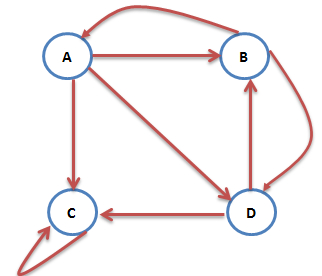
\includegraphics[width=8cm]{fig/Fig1.jpg}
  \caption{陷阱}\label{xj}
\end{figure}

为了避免上述问题,在算法中引入阻尼系数$\alpha$,作为网页随机跳转的概率。PageRank的计算公式也被修正为:
\[PR(p_i)=\alpha\sum_{p_j\in M_{p_i}}\frac{PR(p_j)}{L_({p_j})}+\frac{1-\alpha}{N}\]
其中$N$是网页总数。

阻尼系数$\alpha$可理解为用户继续点击当前网页中的链接的概率,$(1-\alpha)$
为用户通过地址栏``逃离''的概率,$\alpha$一般取值为0.85。根据上面的公式,我们可以计算每个网页的$PR$值,在不断迭代趋于平稳的时候,即为最终结果。

\subsection{实例分析}
在这里,我们先用一个简单的例子来说明PageRank算法,以图~\ref{xj}为例。首先,我们写出该网络的出入链关系,即转移概率矩阵
\[T=\begin{pmatrix}0&1/3&1/3&1/3\\
1/2&0&0&1/2\\
0&0&1&0\\
0&1/2&1/2&0\end{pmatrix}\]

我们用$m$维列向量$P=(PR_1,PR_2,\cdots,PR_m)^T$来记录$m$个网站的$PR$值,则初始$PR$值为$P_0=(1/m,1/m,\cdots,1/m)^T$。根据PageRank算法原理,我们可以给出如下迭代公式:
\[P_{n+1}=\alpha T^TP_n+(1-\alpha)P_0\]
取$\alpha=0.85$,我们有
\[\begin{pmatrix}
PR_1^{(n+1)}\\PR_2^{(n+1)}\\PR_3^{(n+1)}\\PR_4^{(n+1)}\\
\end{pmatrix}=0.85\begin{pmatrix}0&1/2&0&0\\
1/3&0&0&1/2\\
1/3&0&1&1/2\\
1/3&1/2&0&0\end{pmatrix}
\begin{pmatrix}
PR_1^{(n)}\\PR_2^{(n)}\\PR_3^{(n)}\\PR_4^{(n)}\\
\end{pmatrix}+0.15\begin{pmatrix}
1/4\\1/4\\1/4\\1/4
\end{pmatrix}\]
且
\[P_0=(1/4,1/4,1/4,1/4)^T\]

我们运用Matlab编写程序得到$m$个网站的$PR$值
\[P=\begin{pmatrix}
   0.082\ 493\ 125\ 6\\
   0.105\ 866\ 177\ 8\\
   0.705\ 774\ 518\ 8\\
   0.105\ 866\ 177\ 8\\
\end{pmatrix}\]
可见,网页C的质量最高,网页B和D次之,网页A的质量最低。

\subsection{PageRank算法在知乎大V社交网络分析中的运用}

基于上述对PageRank算法的阐述,我们现在将此算法运用到知乎大V的社交网络分析中。

我们运用Matlab编写程序``\texttt{PR.m}'',运行得到200个知乎大V的$PR$值,并储存在文件``\texttt{PR\_Vaule.xlsx}''中。在这里,我们仅给出$PR$值前10名的大V与相应的$PR$值。
\begin{center}
\begin{tabular}{ccc}
\toprule
排序& 知乎大V &  $PR$值\\
\midrule
1 & 黄继新 & 0.0170602\\
2  & 周源 & 0.0136871\\
3 & 张亮	 & 0.0136203\\
4 & Raymond Wang & 0.0120307\\
5 & 张佳玮 & 0.0116971\\
6 & 李淼 & 	0.0110405\\
7 & 负二	 & 0.0107342\\
8 & 马伯庸 & 0.0106872\\
9 & 葛巾	 & 0.0106016\\
10 & keso & 0.0102862\\
\bottomrule
\end{tabular}
\end{center}

我们发现,黄继新的$PR$值最高,这也意味着其在知乎大V的影响力是巨大的。
\newpage
\section{PageRank与其他中心性度量的比较}\label{sec6}
我们以用户的PageRank值作为自变量,将其他中心性归一化后作为因变量,绘制出散点图并进行线性回归,如图~\ref{bj}所示。
\begin{figure}[H]
  \centering
  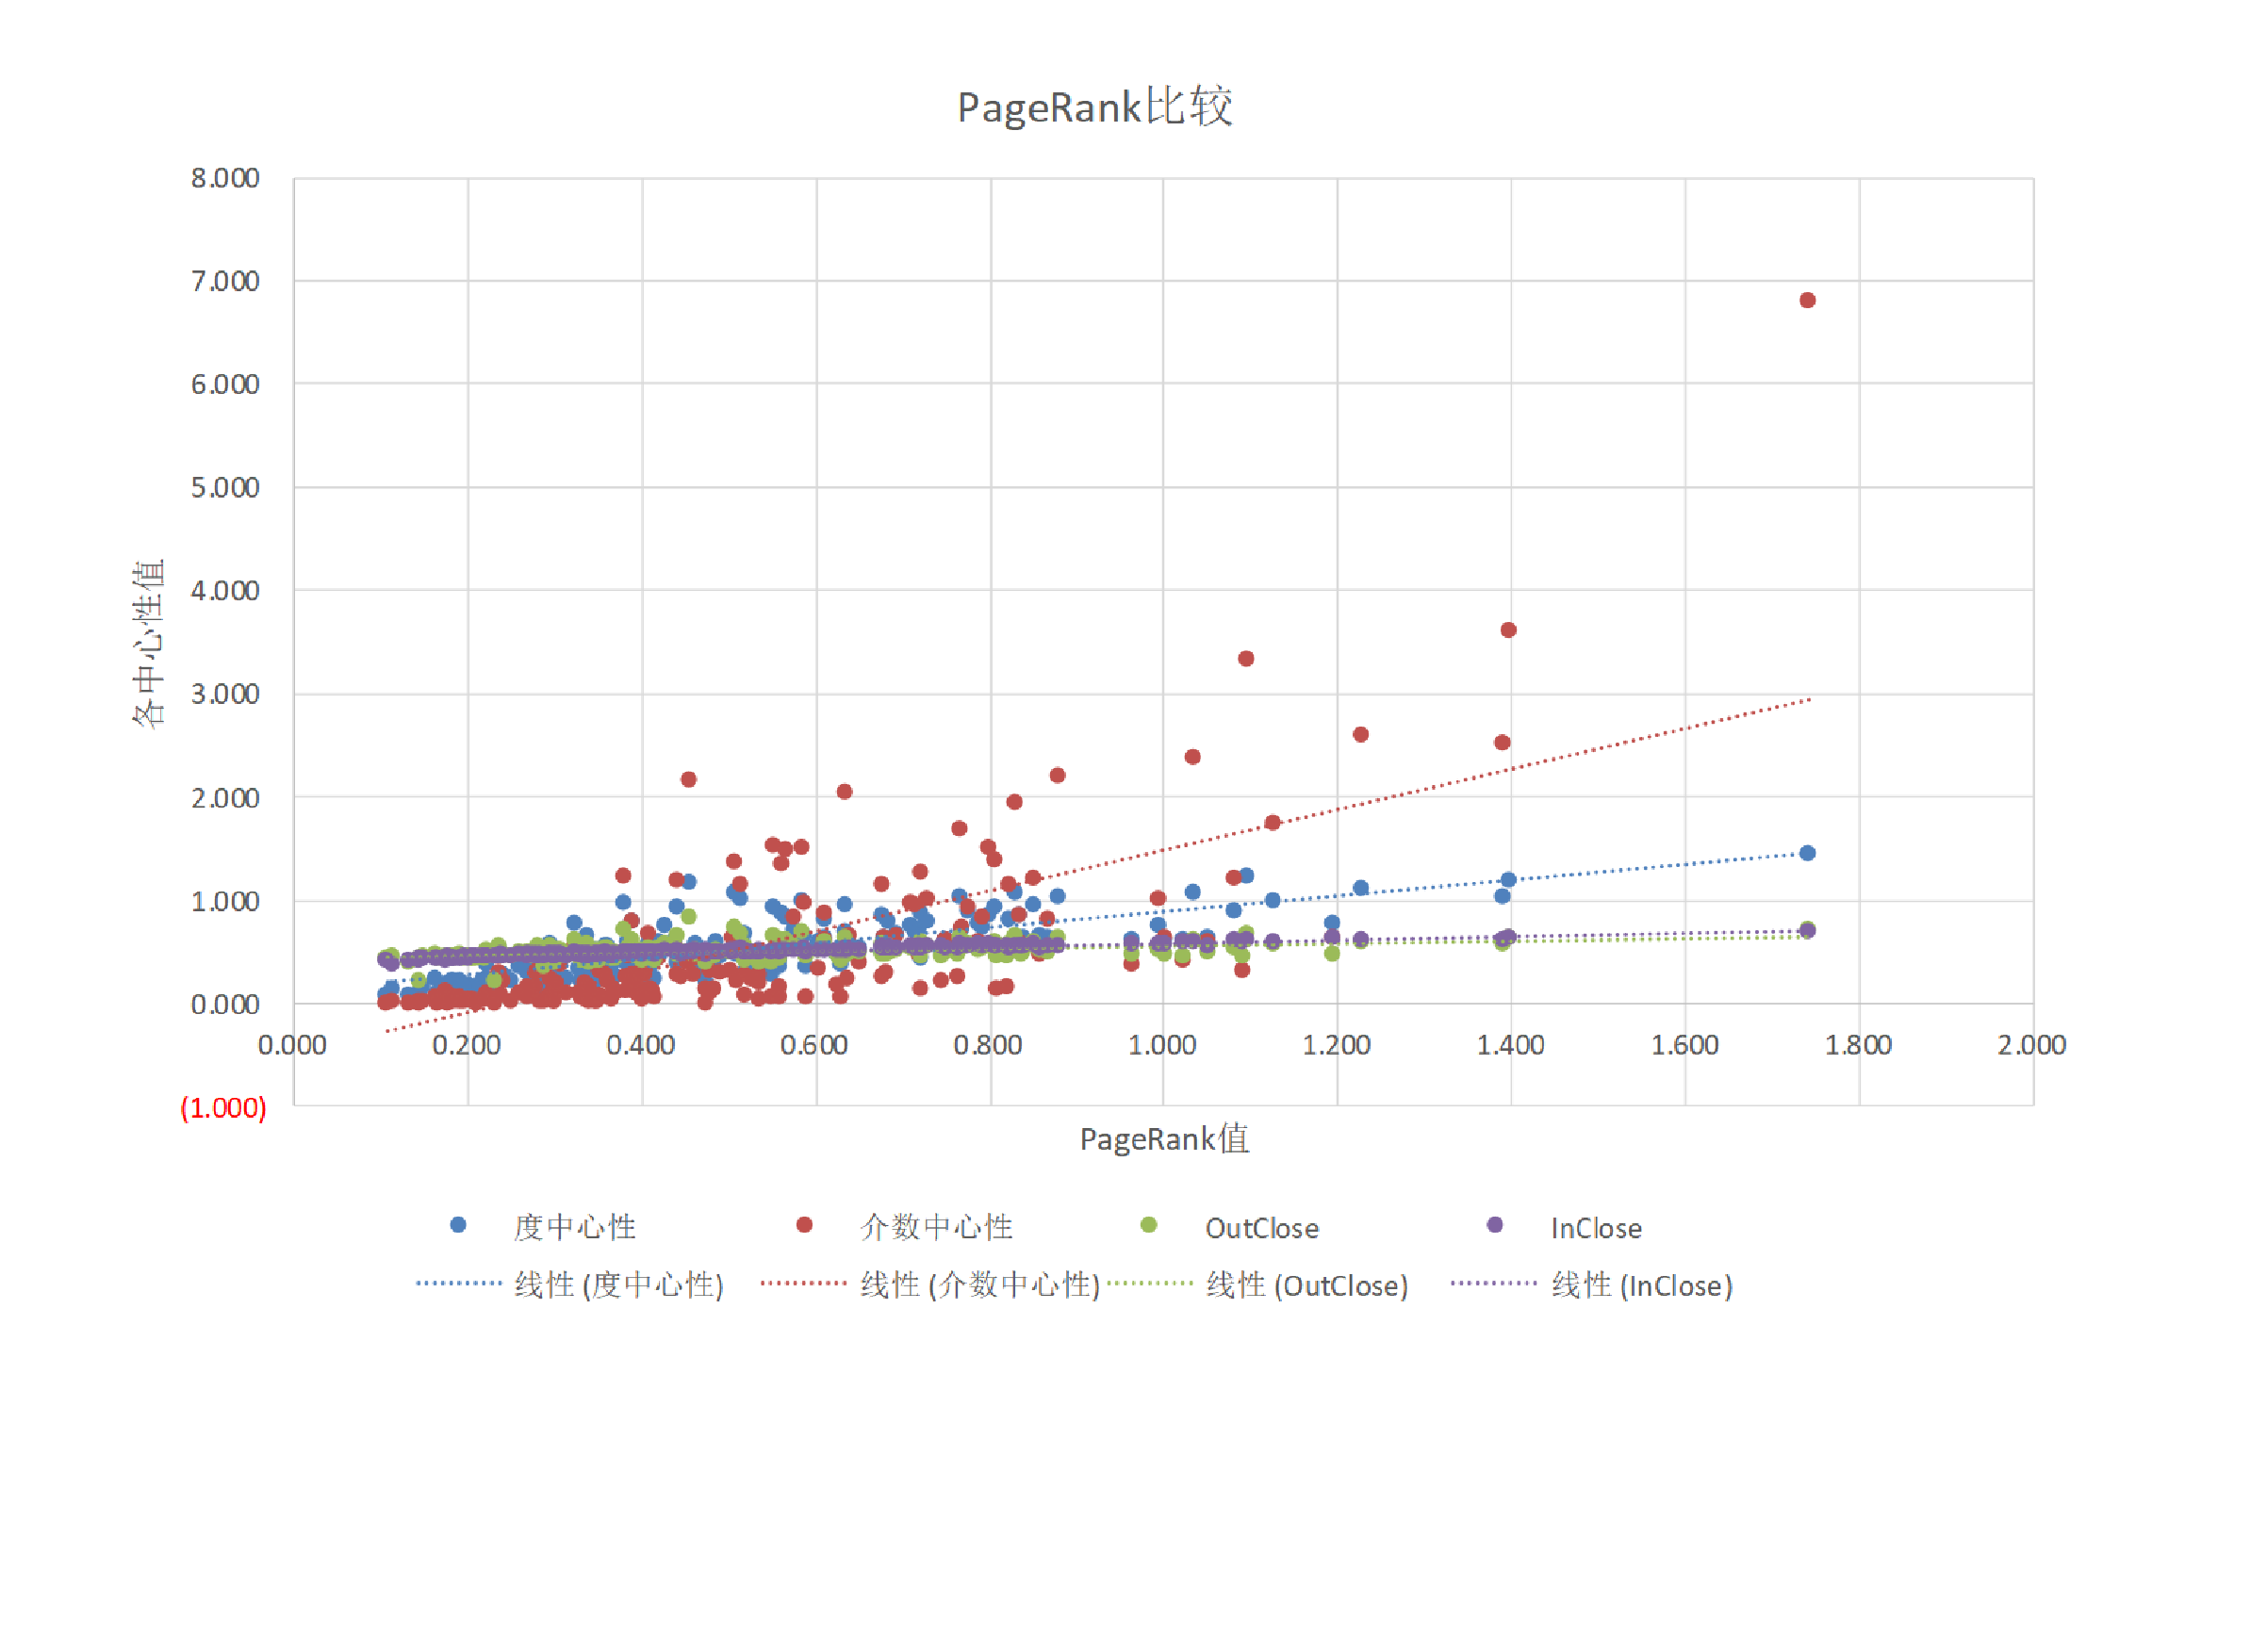
\includegraphics[width=15cm]{fig/PageRank.pdf}
  \caption{以PR值为自变量的散点图}\label{bj}
\end{figure}


从图中可以看出:接近中心性和度中心性都基本上和PageRank值成线性关系,而介数中心性也总体上成正相关关系。

所以,从总体上来说,节点的PageRank值与其出接近中心性、入接近中心性、中介中心性和度中心性这些中心度指标是统计上显著相关的,因此,我们可以认为节点的PageRank值是对节点中心度指标的一种综合。

但我们也能看出有不少人PR值高却介数中心性较低,可见PageRank在衡量节点的枢纽能力上仍有一定局限性,具体原因有待进一步考证。

\newpage
\section{数据分析}\label{sec7}
我们试图通过已获取的用户信息(见文件"\verb"Info_2018_5_26.xlsx"")来进行分析,探索那些PR值较高的用户有哪些特征。结论如下:

\begin{itemize}
\item
整体来看,知乎PR值前五十名的用户中,比例最高的行业为互联网,其次为作家。使用回归分析分析数据可得,PR值与关注者数存在明显正相关,与回答数目和文章的数目无明显正相关关系。

\item
通过分析PR值高的用户特点可以发现,PR值较高的用户大多或具有牢固的某专业知识技能,能够给人提供指导;或文字风格幽默风趣,能写段子;或个性鲜明,能洞察世事,提出与众不同的见解。

\item
PR值超过0.01的用户有14个,男女比12:2。其中从事互联网行业的四个,分别为“周源”、“黄继新”、“张亮”、“李淼”;从事作家行业的有四个,分别为“张佳玮”、“负二”、“马伯庸”、“keso”;从事科研的有两个,分别为“maggie”、“chenqin”;从事法律行业的有一个,为“Raymond Wang”;从事咨询分析行业的有一个,为“葛巾”;从事电子游戏行业的有一个,为“cOMMANDO”。

\item
PR值排名前三的均为知乎的联合创始人或CEO。


\end{itemize}

可见影响知乎上社交的主要因素为个人见识的深浅和个人的表达能力,其中当然不排除吹嘘和捏造的成分。知乎作为一个分享见解、分享故事的问答平台,用户通过为别人提供自己的见解和分享自己的故事来获得更多的读者,进而扩大自己的社交广度。
\end{spacing}
\end{document}
